\documentclass{VUMIFPSkursinis}
\usepackage{algorithmicx}
\usepackage{algorithm}
\usepackage{algpseudocode}
\usepackage{amsfonts}
\usepackage{amsmath}
\usepackage{bm}
\usepackage{caption}
\usepackage{color}
\usepackage{float}
\usepackage{graphicx}
\usepackage{listings}
\usepackage{subfig}
\usepackage{wrapfig}
\usepackage{longtable}

\usepackage{enumitem}
%PAKEISTA, tarpai tarp sąrašo elementų
\setitemize{noitemsep,topsep=0pt,parsep=0pt,partopsep=0pt}
\setenumerate{noitemsep,topsep=0pt,parsep=0pt,partopsep=0pt}

% Titulinio aprašas
\university{Vilniaus universitetas}
\faculty{Matematikos ir informatikos fakultetas}
\department{Programų sistemų katedra}
\papertype{Kursinis darbas}
\title{Paieškos proceso ir jos rezultatų pateikimo vartotojams panaudojamumas VUL Santaros klinikų puslapyje}
\titleineng{The Usability of the Search Process and Presenting its Results to the User for VUH Santaros klinikos website}
\status{3 kurso 3 grupės studentas}
\author{Tomas Kiziela}
% \secondauthor{Vardonis Pavardonis}   % Pridėti antrą autorių
\supervisor{doc. Kristina Lapin}
\date{Vilnius – \the\year}

% Nustatymai
% \setmainfont{Palemonas}   % Pakeisti teksto šriftą į Palemonas (turi būti įdiegtas sistemoje)
\bibliography{bibliografija}

\begin{document}
	
% PAKEISTA	
\maketitle
\cleardoublepage\pagenumbering{arabic}
\setcounter{page}{2}

%TURINYS
\tableofcontents

\sectionnonum{Įvadas}
%Įvade apibūdinamas darbo tikslas, temos aktualumas ir siekiami rezultatai.
%Darbo įvadas neturi būti dėstymo santrauka. Įvado apimtis 1–2 puslapiai.
Šiame darbe tiriami informacijos paieškos architektūros sprendimai leidžiantys palengvinti Vilniaus universiteto ligoninės (VUL) Santaros klinikų internetinio puslapio santa.lt naudojimą. Tyrime bus atsižvelgta į puslapio navigaciją, paieškos procesą bei gautų rezultatų pateikimą.

Kadangi Lietuvos gyventojams internetas lengvai prieinamas, darosi įprasta ieškoti informacijos apie sveikatą ir registruotis pas gydytoją internetu\cite{InternetUseByPublicSAEn}\cite{InternetUseByPublicHKEn}. VUL Santaros klinikos yra viena didžiausių Lietuvos ligoninių. Joje dirba virš 5000 darbuotojų, o per metus gydoma apie 1 milijonas ambulatorinių (ateinančių iš namų) pacientų\cite{VulSkApieMusLt}. Taigi santa.lt puslapis yra vienas iš pirmųjų internetinių resursų, kurį pasiekia vartotojai. Puslapyje turėtų būti lengva surasti ieškomą informaciją, nes tai padės sergantiems priimti sprendimus apie savo sveikatą.

Tačiau dabartinėje sistemoje vartotojai susiduria su panaudojamumo problemomis. Naudojant paieškos sistemą negalima įvesti pilnų žodžių, nes, jeigu galūnė bent kažkiek skirsis, paieška rezultato negražins. Be to, ieškodamas informacijos apie širdies ligas gauni pilną puslapį padėkų, kurios, nors džiugina, užslepia rezultatus kaip širdies ligų gydymo centro kontaktai. Filtravimas nepadeda, nes gražinti rezultatai yra skirstomi į per plačias kategorijas, kuriose padėkos, naujienos ir svetainės esminiai puslapiai tokie kaip „Kontaktai“ ar „Apie mus“ yra vienoje kategorijoje. 

Šio darbo tikslas yra suprojektuoti informacijos architektūrą, kuri leistų pacientams greičiau ir su mažiau paspaudimų rasti aktualią informaciją santa.lt puslapyje. Pacientams aktualu yra registracija pas gydytoją, informacija kaip pasiekti ligoninę ir jos skyrius, informacija apie ligoninės personalą. Galutinis darbo rezultatas - puslapio prototipas, kurio informacijos architektūra leidžia greičiau ir su mažiau paspaudimų rasti aktualią informaciją.

Uždaviniai:
\begin{enumerate}
	\item Identifikuoti vartotojų poreikius remiantis literatūros šaltiniais ir internetinių puslapių lankomumo informacija
	\item Išskirti lyginimo kriterijus remiantis literatūros šaltiniais
	\item Atlikti puslapio panaudojamumo analizę
	\item Paruošti sprendimo variantus
	\renewcommand*{\theenumii}{\theenumi.\arabic{enumii}}
	\renewcommand{\labelenumii}{\theenumii}
	\begin{enumerate}
		\item Remiantis panašiais puslapiais ir literatūros šaltiniais išskirti alternatyvius sprendimus
		\item Sukurti sprendimo variantų maketus
		\item Palyginti maketus
		\item Sukurti galutinio sprendimo prototipą
	\end{enumerate}
	\item Išskirti detalius reikalavimus galutinio sprendimo įgyvendinimui
	\item Atlikus literatūros analizę išskirti technologijas padedančias įgyvendinti galutinį sprendimą
\end{enumerate}



\section{Vartotojų poreikių analizė}
Tyrimai nurodo, kad Europoje daugiau nei pusė žmonių bent kartą metuose ieško informacijos apie sveikatą internetu \cite{EuCitizDigHealthEn}, taigi naudotojams aktualu internetinių puslapių panaudojamumas. Nagrinėjant santa.lt puslapio srautą randama, kad naudotojai dažniausiai ateina iš (5,5\%) ir keliauja į (10,4\%) sergu.lt (neįskaitant 19,1\% ateinančių iš google.com ir 21,8\% keliaujančių į google.com)\cite{AlexaSantaEn}. Taigi galima matyti, kad šių puslapių vartotojai iš dalies sutampa ir būtų naudinga atsižvelgti į tai, kokią įtaką daro vienas kitam. Sergu.lt puslapis skirtas išankstinei visų Lietuvos pacientų registracijai internetu. Tai, kad 1 iš 10 santa.lt vartotojų tiesiogiai pereina į sergu.lt puslapį leidžia tikėti, kad vienas iš vartotojų poreikių yra rasti nuorodą į registraciją pas gydytoją. Santa.lt „Kaip mus rasti“ skyrelį vartotojai yra aplankę 1,2 milijonus kartų\cite{VulSkKaipMusRastiLt}, 2 kartus daugiau nei skyrelį „Apie mus“\cite{VulSkApieMusLt}, iš to galima daryti prielaidą apie kitą vartotojų poreikį - sužinoti apie ligoninės klinikų pasiekiamumą.

Norint daugiau sužinoti apie vartotojų poreikius buvo atlikta apklausa kartu su panaudojamumo testavimu (n = 5). Dalyvių buvo prašoma atlikti tipinio naudojimo užduotis, o po užduočių buvo užduodami klausimai apie sistemos naudojimą. Iš atsakymų matyti:
\begin{enumerate}
%\item Naudotojai vidutiniškai užtrunka 1 minutę rasti skyriaus adresą
%\item Naudotojai vidutiniškai užtrunka 52 sekundes rasti registraciją pas gydytoją, kai negalima eiti į pagrindinį puslapį.
%\item Visi naudotojai nerado ligoninės skyrių ir registracijos per paiešką
\item 4 iš 5 naudotojų mano, kad sistemoje turėtų būti galima greičiau atlikti kai kurias užduotis
\item 3 iš 5 naudotojų mano, kad informacija galėtų būti geriau struktūrizuota
\item Visi naudotojai buvo nepatenkinti paieškos sistema
\end{enumerate}

Apklausa parodė, kad vartotojai nėra patenkinti dabartine sistema. Norint toliau nagrinėti sistemos trūkumus ir privalumus reikia surasti lyginimo kriterijus, pagal kuriuos bus galima palyginti senos ir naujos sistemos panaudojamumą.



\section{Sistemų lyginimo kriterijai}
Panaudojamumo inspekcija gali būti atlikta įvairiais metodais. Empiriniai metodai yra plačiausiai naudojami\cite{NielsenUsabilityEn}, tačiau reikalauja daug žmonių norint gauti patikimą rezultatą, todėl atliktas vienas iš analitinių metodų. Dėl paprastumo pasirinkta naudoti neformaliausią metodą - euristinį vertinimą, šiuo naudojantis nereikia turėti eksperto žinių. Norint surasti optimalų sprendimą reikia turėti objektyvius kriterijus, pagal kuriuos galima lyginti skirtingus sprendimo variantus. Šiam tyrimui naudojamos David Travis gairės, kuris nuo 1989 metų dirba vartotojo patirties srityje ir yra parašęs dvi knygas apie panaudojamumą. Savo tinklapyje jis turi daug gairių, tačiau šiam tyrimui aktualios gairės paieškos ir informacijos architektūros vertinimui. Jo gairės suformuluotos teiginių pavidalu ir vertinant puslapį jos yra žymimos kaip tenkinamos arba netenkinamos\cite{SearchGuidelinesEn}\cite{NavigationAndIAGuidelinesEn} (\ref{PaieškosLentelėPrad} ir \ref{navigacijosirIAlentelėPrad} lentelės). Alternatyviai būtų galima naudoti Jacob Nielsen euristikas, kuris vadinamas tinklapių projektavimo guru, tačiau autoriui atrodo, kad David Travis gairės leidžia objektyviau įvertinti puslapį, nes tereikia atsakyti į taip arba ne klausimus, o ne įvertinti skalėje nuo 0 iki 3. Kitas gairių privalumas yra tai, kad klausimai gan konkretūs ir lengvai patikrinami, o euristikos gan plačios ir reikia gerai žinoti jų prasmę. Gairės vistiek nėra tobulos, nes tinklapio projektavime galima prioritizuoti tam tikras gaires virš kitų, siekant specifiško rezultato, tačiau šį faktą ignoruosime ir vertinsime pagal išpildytų gairių skaičių.

Naudojant pasirinktus kriterijus galima įvertinti dabartinės sistemos panaudojamumo būseną ir palyginti su alternatyviais sprendimo maketais.



\section{Puslapio panaudojamumo analizė}
Norint išsiaiškinti dabartinės sistemos panaudojamumo būseną autorius atliko panaudojamumo inspekciją pagal praėjusiame skyriuje išvardintus kriterijus.

\begin{center}
\begin{tabular}{ |p{13,5cm}|p{2cm}| } 
 \hline
	Gairė & Ar tenkina \\ \hline
	1) Pagrindinė paieška lengvai valdoma & netenkina \\ \hline
	2) Paieškos rezultatų puslapis naudotojui rodo, ko buvo ieškota, ir yra lengva pakeisti ir pakartoti užklausą & tenkina \\ \hline
	3) Paieškos rezultatai yra aiškūs, naudingi ir reitinguojami pagal atitikimą užklausai & netenkina \\ \hline
	4) Paieškos rezultatų puslapis aiškiai parodo kiek rezultatų gražinta ir rezultatų skaičius per puslapį gali būti reguliuojamas naudotojo & tenkina \\ \hline
	5) Jei negražinamas nei vienas rezultatas, sistema pasiūlo idėjų ar nustatymų pagerinti užklausai atsižvelgiant į atpažįstamas įvesties problemas & netenkina \\ \hline
	6) Paieška dailiai susitvarko su tuščia užklausa & tenkina \\ \hline
	7) Dažniausios užklausos gražina naudingus rezultatus & netenkina \\ \hline
	8) Paieškos sistema turi šabloną arba patarimus kaip ją deramai naudoti & netenkina \\ \hline
	9) Puslapis turi pajėgesnę paieškos sąsają leidžiančią naudotojams patikslinti užklausas & tenkina \\ \hline
	10) Paieškos rezultatų puslapis nerodo besikartojančių rezultatų & tenkina \\ \hline
	11) Paieškos laukas pakankamai ilgas dažniausių užklausų ilgiams & netenkina \\ \hline
	12) Paieška apima visą interneto svetainę, o ne tik jos dalį & tenkina \\ \hline
	13) Jei svetainė leidžia naudotojams sudaryti sudėtingą paiešką, šios paieškos gali būti išsaugojamos ir kartojamos reguliariai & tenkina \\ \hline
	14) Paieškos sąsaja padėta, naudotojams įprastoje vietoje (viršuje dešinėje) & tenkina \\ \hline
	15) Paieškos laukas ir jo kontrolės aiškiai pavadintos & tenkina \\ \hline
	16) Puslapis palaiko paieškos strategiją ir naršymo strategiją & netenkina \\ \hline
	17) Paieškos sritis aiškiai parašyta paieškos rezultatų puslapyje ir naudotojai gali ją susiaurinti & tenkina \\ \hline
	18) Paieškos rezultatų puslapis atvaizduoja naudingą meta informaciją (informacija apie informaciją), kaip dokumento dydis, dokumento sukūrimo data ir failo tipas & tenkina \\ \hline
	19) Paieškos sistema automatiškai patikrina rašybą ir ieško daugiaskaitinių formų ir sinonimų & netenkina \\ \hline
	20) Paieškos sistema leidžia ieškoti panašių rezultatų („daugiau tokių“) &  \\ \hline
\end{tabular}
\captionof{table}{Paieškos panaudojamumo gairių vertinimo lentelė pradiniam puslapiui}\label{PaieškosLentelėPrad}
\end{center}

\vspace{1cm}

\begin{center}
\begin{longtable}{ |p{13,5cm}|p{2cm}| } 
 \hline
	Gairė & Ar tenkina \\ \hline
	1) Yra patogus ir akivaizdus būdas judėti tarp susijusių puslapių ir skyrių ir yra lengva grįžti į pagrindinį puslapį & netenkina \\ \hline
	2) Informacija, kurios naudotojams dažnai prireikia yra lengvai pasiekiama iš daugumos puslapių & tenkina \\ \hline
	3) Navigacijos pasirinkimai išrikiuoti pačiu racionaliausiu arba užduočiai orientuotu būdu &  \\ \hline
	4) Navigacijos sistema plati ir sekli (daug meniu elementų), o ne gili (daug meniu lygių)  &  \\ \hline
	5) Paprasta, aiškaus modelio svetainės struktūra be nereikalingų lygių &  \\ \hline
	6) Pagrindiniai puslapio skyriai pasiekiami iš bet kurio puslapio ir nėra aklaviečių &  \\ \hline
	7) Navigacijos skirtukai patalpinti puslapio viršuje ir atrodo kaip paspaudžiamos versijos realaus pasaulio skirtukų &  \\ \hline
	8) Yra svetainės žemėlapis, kuris suteikia svetainės turinio apžvalgą &  \\ \hline
	9) Svetainės žemėlapį galima pasiekti iš bet kurio puslapio &  \\ \hline
	10) Svetainės žemėlapis suteikia glaustą svetainės apžvalgą, o ne pernaudotą navigacijos meniu ar sąrašą kiekvienos temos &  \\ \hline
	11) Suteikiamas geras navigacijos grįžtamasis ryšys (rodoma, kur randiesi puslapyje) &  \\ \hline
	12) Kategorijų pavadinimai tiksliai apibūdina informaciją viduje &  \\ \hline
	13) Nuorodos ir navigacijos pavadinimai susidaro iš raktinių žodžių, kurių naudotojai ieškos bandydami atlikti užduotį &  \\ \hline
	14) Terminologija ir susitarimai (kaip nuorodų spalvos) (maždaug) atitinka bendrą interneto naudojimą &  \\ \hline
	15) Nuorodos atrodo taip pačiai skirtingose svetainės dalyse &  \\ \hline
	16) Produktų puslapiai turi nuorodas į panašius arba papildomus produktus, kad paskatinti kryžminį pardavimą (angl. cross-selling) &  \\ \hline
	17) Navigacijos elementams ir hiperteksto nuorodoms naudojami terminai yra nedviprasmiški ir be žargono &  \\ \hline
	18) Naudotojai gali rikiuoti ir filtruoti katalogo puslapius (pagal kainą arba populiarumą) &  \\ \hline
	19) Matomi pasikeitimai, kai naudotojas užveda kursorių ant kažko paspaudžiamo (neįskaitant kursoriaus pasikeitimų) &  \\ \hline
	20) Svarbus turinys pasiekiamas iš daugiau nei vienos nuorodos (naudotojams gali reikėt skirtingų nuorodų pavadinimų) &  \\ \hline
	21) Puslapiai skirti tik navigacijai (pavyzdžiui pradinis puslapis) gali būti peržiūrimi be slinkimo &  \\ \hline
	22) Hipertekso nuorodos, kurios sukelia veiksmus (pavyzdžiui siuntimą) aiškiai skiriasi nuo nuorodų, kurios veda į kitą puslapį &  \\ \hline
	23) Svetainė leidžia naudotojui kontroliuoti sąveikos greitį ir eiliškumą &  \\ \hline
	24) Visuose puslapiuose yra aiškiai pažymėti išėjimai leidžiantys naudotojui pabėgti iš esamos užduoties be papildomo dialogo &  \\ \hline
	25) Svetainė neišjungia naršyklės „atgal“ mygtuko ir „atgal“ mygtukas visada matomas naršyklės įrankių juostoje &  \\ \hline
	26) Paspaudus „atgal“ mygtuką naudotojas visada gražinamas į puslapį, iš kurio atėjo &  \\ \hline
	27) Nuoroda į prekių krepšelį ir atsiskaitymą matomi visuose puslapiuose &  \\ \hline
	28) Jeigu puslapis sukuria naujus langus, jie neklaidina naudotojo (jie dialogo lango dydžio ir lengvai uždaromi) &  \\ \hline
	29) Meniu instrukcijos, nurodymai ir žinutės atsiranda toje pačioje vietoje visuose puslapiuose &  \\ \hline
	\caption{Navigacijos ir informacijos architektūros panaudojamumo gairių vertinimo lentelė pradiniam puslapiui}\label{navigacijosirIAlentelėPrad}
\end{longtable}
\end{center}

%Medžiagos darbo tema dėstymo skyriuose pateikiamos nagrinėjamos temos detalės:
%pradinė medžiaga, jos analizės ir apdorojimo metodai, sprendimų įgyvendinimas,
%gautų rezultatų apibendrinimas. Šios dalies turinys labai priklauso nuo darbo
%temos. Skyriai gali turėti poskyrius ir smulkesnes sudėtines dalis, kaip
%punktus ir papunkčius.

%Medžiaga turi būti dėstoma aiškiai, pateikiant argumentus. Tekstas dėstomas
%trečiuoju asmeniu, t.y. rašoma ne „aš manau“, bet „autorius mano“, „autoriaus
%nuomone“. Reikėtų vengti informacijos nesuteikiančių frazių, pvz., „...kaip jau
%buvo minėta...“, „...kaip visiems žinoma...“ ir pan., vengti grožinės literatūros
%ar publicistinio stiliaus, gausių metaforų ar panašių meninės išraiškos
%priemonių.

\section{Sprendimo variantai}

\subsection{Alternatyvieji sprendimai}
Bandant sukurti sprendimo maketus bus remiamasi jau egzistuojančiais ligoninių puslapiais, kurie atitinka prisitaikančio dizaino (angl. responsive design) principus. Prisitaikantis dizainas leidžia turėti vieną puslapį, kuris prisitaiko prie įvarių ekrano formų ir dydžių\cite{RWDEn}. Pavyzdiniai puslapiai parinkti iš didmiesčių ligoninių, Vilniaus, Kauno ir Niujorko. Autoriaus subjektyvia nuomone Kauno ligonės puslapis yra ypač geras pavyzdys. Sumuštinio meniu, registracijos mygtukas ir paieška yra geriausiai matomoje vietoje, naudojami dideli mygtukai su aiškiais užrašais bei kontrastingos spalvos, taigi net žmonėms su prastu regėjimu turėtų būti patogu naudotis (\ref{img:kaunomobile} pav.).

Sprendimo maketai bus kuriami naudojant Balsamiq programinę įrangą, nes ji leidžia greitai sukurti grubų maketą ir autoriui jau tekę ja naudotis. Galutinio sprendimo maketas bus kuriamas su Axure RP 9, nes tai leis sukurti maketą, kuris panašesnis į galutinį rezultatą.

\subsection{Sprendimo maketai}
\subsubsection{Pirmas maketas}

\subsubsection{Antras maketas}

\subsection{Maketų palyginimas}
\subsection{Galutinio sprendimo prototipas}

\section{Reikalavimai galutinio sprendimo įgyvendinimui}
\section{Technologijos galutinio sprendimo įgyvendinimui}

\sectionnonum{Rezultatai ir išvados}

%Rezultatų ir išvadų dalyje turi būti aiškiai išdėstomi pagrindiniai darbo
%rezultatai (kažkas išanalizuota, kažkas sukurta, kažkas įdiegta) ir pateikiamos
%išvados (daromi nagrinėtų problemų sprendimo metodų palyginimai, teikiamos
%rekomendacijos, akcentuojamos naujovės).


%% PAKEISTAS PAVADINIMAS Į 'Šaltiniai'
\printbibliography[heading=bibintoc, title=Šaltiniai]  % Šaltinių sąraše nurodoma panaudota
% literatūra, kitokie šaltiniai. Abėcėlės tvarka išdėstomi darbe panaudotų
% (cituotų, perfrazuotų ar bent paminėtų) mokslo leidinių, kitokių publikacijų
% bibliografiniai aprašai.  Šaltinių sąrašas spausdinamas iš naujo puslapio.
% Aprašai pateikiami netransliteruoti. Šaltinių sąraše negali būti tokių
% šaltinių, kurie nebuvo paminėti tekste.

% \sectionnonum{Sąvokų apibrėžimai}
%\sectionnonum{Santrumpos}
%Sąvokų apibrėžimai ir santrumpų sąrašas sudaromas tada, kai darbo tekste
%vartojami specialūs paaiškinimo reikalaujantys terminai ir rečiau sutinkamos
%santrumpos.

\appendix  % Priedai
% Prieduose gali būti pateikiama pagalbinė, ypač darbo autoriaus savarankiškai
% parengta, medžiaga. Savarankiški priedai gali būti pateikiami ir
% kompaktiniame diske. Priedai taip pat numeruojami ir vadinami. Darbo tekstas
% su priedais susiejamas nuorodomis.

\section{Dabartinio puslapio grafinė vartotojo sąsaja}
\begin{figure}[H]
    \centering
    
\includegraphics[scale=0.6]{img/RegistracijosAklavietė}
    \caption{Registracijos aklavietė}
    \label{img:registracija}
\end{figure}

\begin{figure}[H]
    \centering
    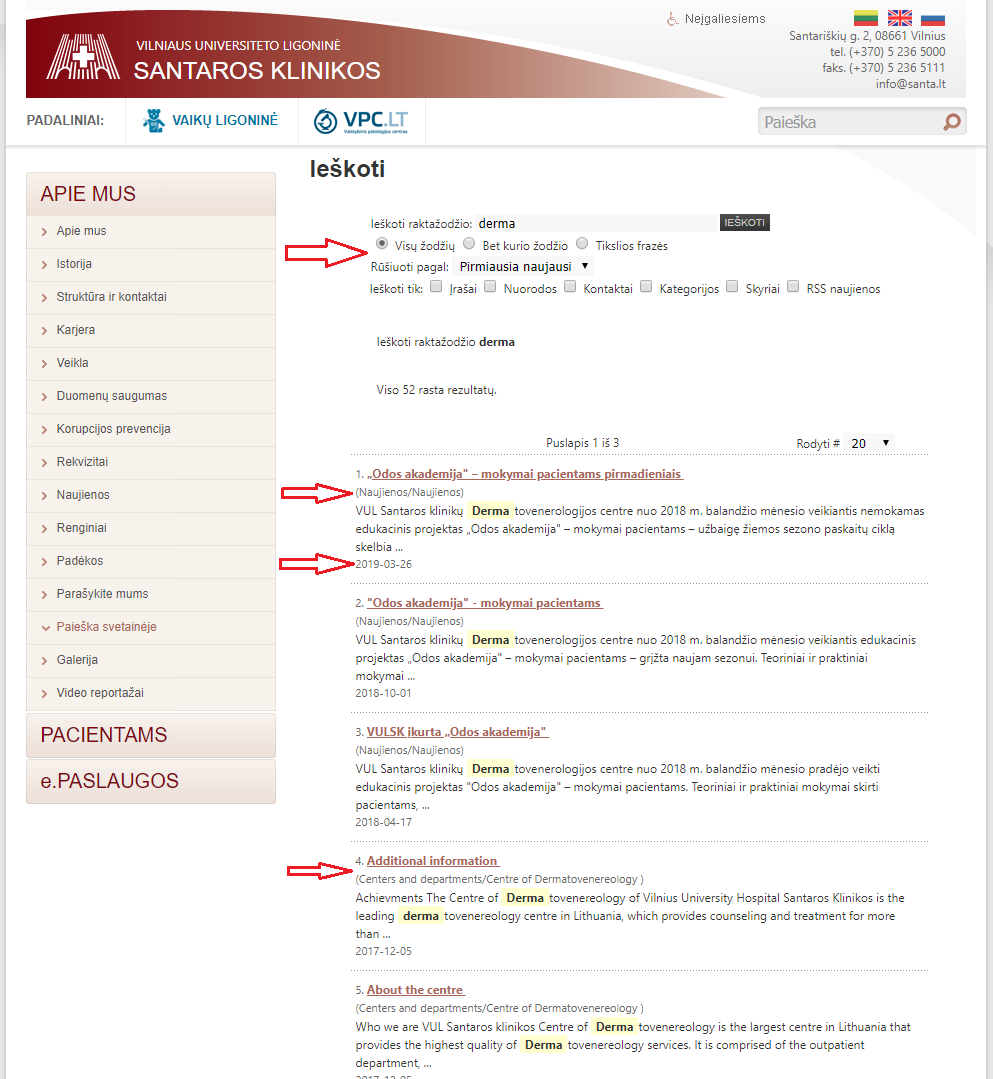
\includegraphics[scale=0.6]{img/PaieškosRezultatai}
    \caption{Paieška ir rezultatai}
    \label{img:paieškarez}
\end{figure}

\section{Puslapių atvaizdavimas ant mobilaus įrenginio}
\begin{figure}[H]
    \centering
    \begin{minipage}{.5\textwidth}
    	\centering
    	
\includegraphics[scale=0.12]{img/SantaMobile}
    	\caption{Santa.lt ant mobilaus įrenginio}
    	\label{img:santamobile}
    \end{minipage}%
    \begin{minipage}{.5\textwidth}
    	\centering
    	
\includegraphics[scale=0.12]{img/VmklMobile}
    	\caption{Vmkl.lt ant mobilaus įrenginio}
    	\label{img:vmklmobile}
    \end{minipage}
\end{figure}

\begin{figure}[H]
    \centering
    \begin{minipage}{.5\textwidth}
    \centering
    
\includegraphics[scale=0.12]{img/KaunoMobile}
    \caption{kaunoligonine.lt ant mobilaus įrenginio}
    \label{img:kaunomobile}
    \end{minipage}%
\begin{minipage}{.5\textwidth}
    \centering
    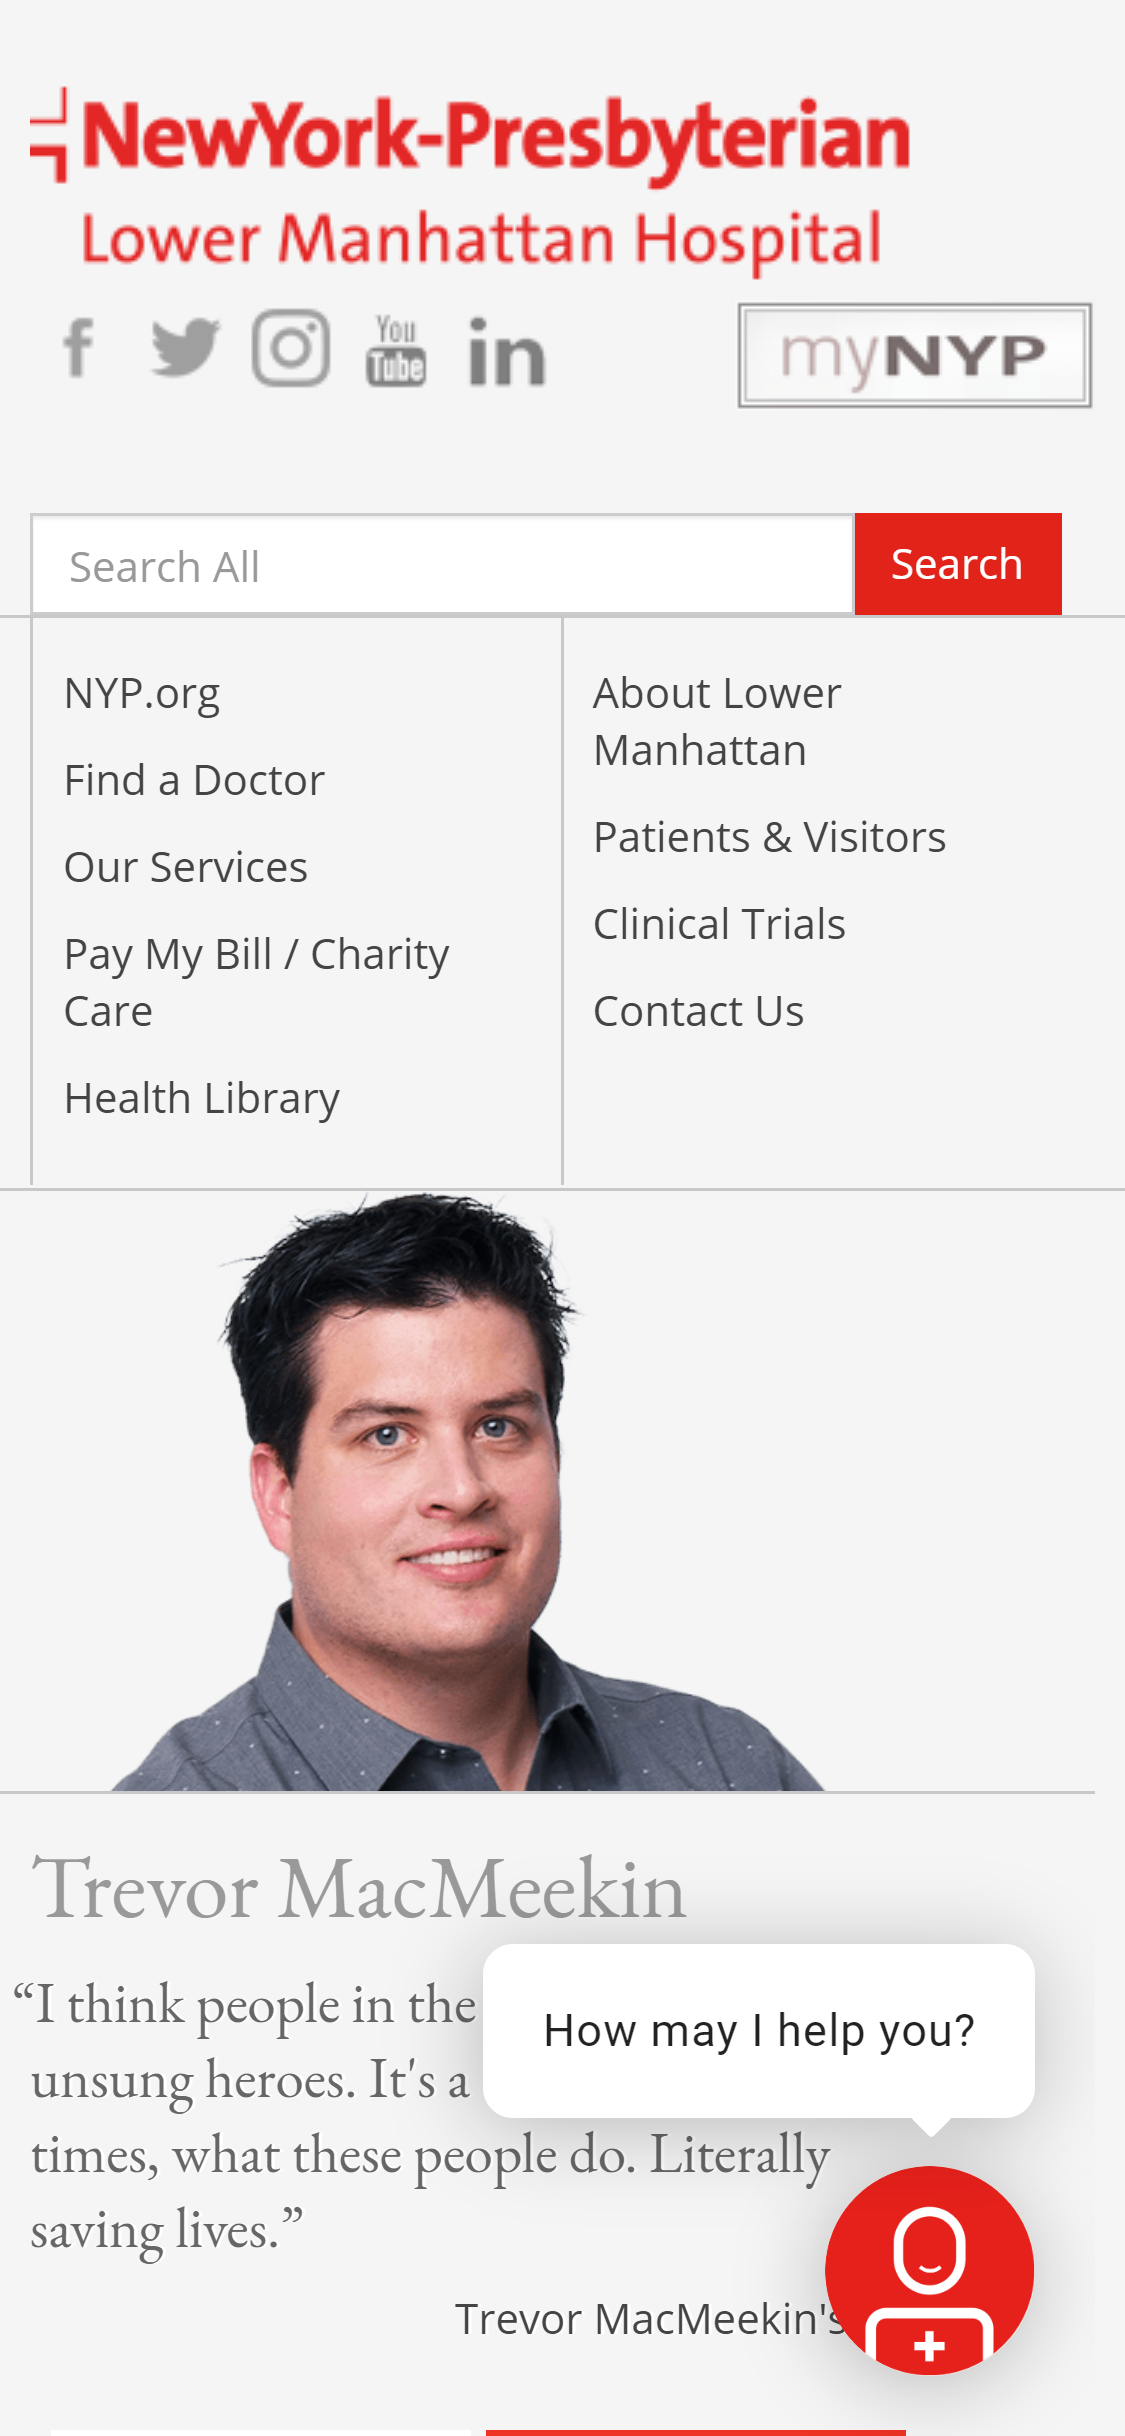
\includegraphics[scale=0.12]{img/NypMobile}
    \caption{nyp.org ant mobilaus įrenginio}
    \label{img:nypmobile}
    \end{minipage}
\end{figure}


%\section{Eksperimentinio palyginimo rezultatai}
% tablesgenerator.com - converts calculators (e.g. excel) tables to LaTeX
%\begin{table}[H]\footnotesize
%  \centering
%  \caption{Lentelės pavyzdys}
%  {\begin{tabular}{|l|c|c|} \hline
%    Algoritmas & $\bar{x}$ & $\sigma^{2}$ \\
%    \hline
%    Algoritmas A  & 1.6335    & 0.5584       \\
%    Algoritmas B  & 1.7395    & 0.5647       \\
%    \hline
%  \end{tabular}}
%  \label{tab:table example}
%\end{table}

\end{document}
